\documentclass[conference]{IEEEtran}
\IEEEoverridecommandlockouts
% The preceding line is only needed to identify funding in the first footnote. If that is unneeded, please comment it out.
\usepackage[square]{natbib}
\setcitestyle{numbers}
\usepackage{amsmath,amssymb,amsfonts}
\usepackage{algorithmic}
\usepackage{graphicx}
\usepackage{textcomp}
\usepackage{cleveref}
\usepackage{diagbox}

\usepackage{xcolor}
\def\BibTeX{{\rm B\kern-.05em{\sc i\kern-.025em b}\kern-.08em
    T\kern-.1667em\lower.7ex\hbox{E}\kern-.125emX}}
\begin{document}
  
  \title{Social Conventions Developed by Multi Agent Systems Using Reinforcement Learning}
  
  \author{\IEEEauthorblockN{Daniel Aaron Salwerowicz}
    \IEEEauthorblockA{\textit{Institutt for datateknologi og beregningsorienterte ingeniørfag} \\
      \textit{Arctic University of Norway, Narvik}\\
      Narvik, Norway \\
      dsa014@post.uit.no}
  }

\maketitle

\begin{abstract}
  In this report I describe my research related to developing a system with self driving taxis that operate in an imaginary city picking up passengers after cinema, opera, and restaurant close. Before that I have simulated simpler models to learn how to handle similar problems and study the emergent social conventions.
\end{abstract}

\begin{IEEEkeywords}
  Reinforcement learning, Erev-Roth model, Q-learning, Multi Agent Systems
\end{IEEEkeywords}

\section{Introduction}
This research project revolved around studying emerging social conventions developed by agents in a Multi Agent System (MAS) that was trained using reinforcement learning methods like Q-Learning and Erev-Roth model. My goal was to see whether or not they will be able to reach a form of social convention, if it was stable, and if it was better than a convention developed by zero intelligence agents.

To begin with I focused on a simple problem where I learned two cars to cross a bridge where only one could cross the bridfe at time. Then I went over to study a group of cars that would cross a bridge that could support only 5 cars at any given point before collapsing. My last task was the most interesting, there I studied behaviour of self driving taxis that would pick up passengers from three different locations and would haggle for the price.


\section{Problem specification}
First problem is quite simple, one car is placed on each end of the bridge. Bridge can only allow one bridge to cross it, and the crossing takes ten minutes. Cars cannot see eachother and as such they need to decide whether to drive or not without knowing what the other did. If both of them decide to cross the brige in the same timeslot then they will crash, while waiting will cost them $10$ minutes extra. In my simulation both of them need to cross the bridge before they can start again. This is of course a continous play, so they will cross the brigde a lot of times.

Second problem was a bit more advanced, where there were more cars ($15$ in my case, though it can be easily changed) who would try to cross the bridge. This time they all started from the same end of the bridge so crashing into eachother was not a problem, however the bridge can only support 5 cars at the same time. As such they need to learn when to cross the bridge, when they know the amount of cars on the bridge, but do not know the capacity.

Last task revolved around auction systems where the self driving cars were used as taxis and they would drive around picking up people from cinema, opera and restaurant. Normally it would happen smoothly where each passenger would pay a fixed price per minute driven. However there was often a surge of passenger when one of these establishments closed and if there were too few cars to take care of the demand they would start initiating auction. Auction itself is a simple English Auction where each passenger would have a certain upper limit on how much he will bid, while taxi had a lower limit. They would be randomly paired and if taxi asked for less than what the passenger would pay then they would be paired together and drive off, if ther didn't strike a deal then they would try again with other agents. Of course there can be up to $4$ passengers that would ride the taxi at the same time, so that would lessen the demand faster.

\section{Methods applied}
If the first case I used simple Q-Learning algorithm where I put up a reward matrix (R-matrix) with values shown in \cref{tab:RTablePart1}. These were used to build a Q-matrix that would inform its further actions. I have also set up a check that if both cars chose to drive in the same time slot then they would be punished by deduction of $200$ points, instead of getting a reward of $100$ points given for driving.

Formula for updating values in Q-matrix is shown in \cref{eq:qAlgortihm}, where $\alpha$ stands for learning factor that can vary between $0-1$, $\gamma$ stands for discount factor with same bounds as $\alpha$, $Q_{old}(s_t,a_t)$ is chosen to be the maximal reachable q-value from new state, and $r_t$ stands for reward given by R-matrix or the rules. 

\begin{equation}
Q_{new}(s_t,a_t) = \alpha \left(r_t + \gamma Q(s_{t+1}, a) - Q_{old}(s_t,a_t) \right)
\label{eq:qAlgortihm}
\end{equation}

\begin{table}[htbp]
  \centerline{
    \begin{tabular}{|l|l|l|}
      \hline
      \diagbox{Action}{State}& Wait & Drive \\ \hline
      Wait  & -10  & -10   \\ \hline
      Drive & 100  & 100   \\ \hline
    \end{tabular}}
  \caption{Reward matrix for cars in first problem.}
  \label{tab:RTablePart1}
\end{table}

In the case of the other problem faced I chose to employ Q-learning algorithm once again in this case my reward matrix is simply made up of two values, $-1$ point for waiting one minute, $100$ points for driving over and $-200$ points for collapsing the bridge. The Q-matrix itself is a vector of length six for a bridge that can only support five cars. However I have set up the problem in such a way that I can change a lot of parameters involved here. These are: number of cars in simulation, number of cars approaching the bridge in given timestep (decided by $\lambda$ in Poisson distribution), speed of cars, lenght of bridge, maximal amount of cars at the bridge.

In this case cars would drive up to bridge and decide each minute if they want to cross the bridge or not, knowing how many cars there are on the bridge at given moment. I chose to allow every car waiting in queue to decide to cross, even if the car before it has decided to wait. I also chose to only punish the car that lead to bridge collapsing, not the other cars that were on the bridge during collapse.

In the last problem I employed Erev-Roth model to  learn my cars instead of Q-learning as I was tasked with using it. In this case as I lacked the time, I went for a simple solution where I assume that all taxis and passengers are in auction, regardless of demand. Each taxi and passenger start with a set propensity for choosing to lower or raise their demand/offer. Propensities are updated by a simple formula shown in \cref{eq:ErevRoth}, where $q_j(t)$ represents propensity for action $j$ at time $t$, while $\phi$ is a recency parameter, and $r$ is the reward. After each update propensities are balanced to always sum up to 1. Those are then used as probabilities for choosing whether to raise or lower their bids.

\begin{equation}
q_j(t+1) = (1-\phi) \cdot q_j(t) + r
\label{eq:ErevRoth}
\end{equation}

In all cases the zero intelligence agents choose their actions randomly.

\section{Results}
In the case of first problem both cars learned quickly to reach a mutual agreement where one car would simply drive first, while the other one would wait for him to cross and then drive afterwards. This is by far not a perfect convention as one car becomes the "alpha" car, never waiting for the other thus getting better score than the "beta" car that would always wait first and lose ten minutes. 

However it is a social convention nonetheless and it is quite stable one at that. Cars learn quite quickly to not collapse the bridge and always end up with an overall increasing score, as shown in \cref{fig:ScoresPart1}. One can also see the scores for zero intelligence agents. Their scores are overall decreasing even if sometimes by pure chance they manage to increase it for a while. Reason for their close relation is caused by the way I set up my simulation where instead of each decision being an isolated encounter I chose to set it up in such a way that I wait untill both cars have crossed bridge before letting them drive again.

\begin{figure}[htbp]
  \centerline{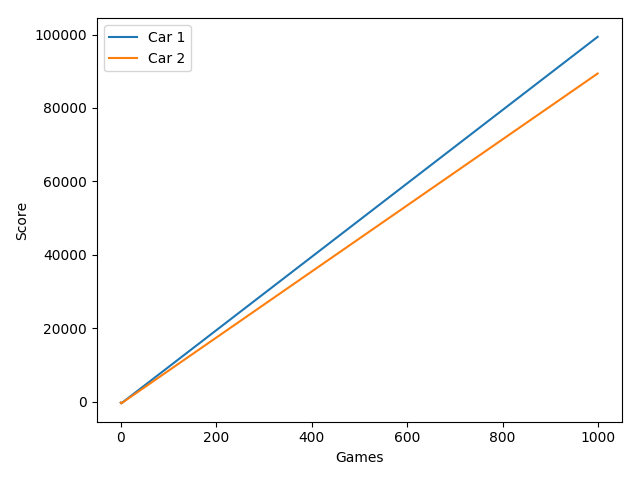
\includegraphics[width=.4\textwidth]{Part1_QLearning}}
  \centerline{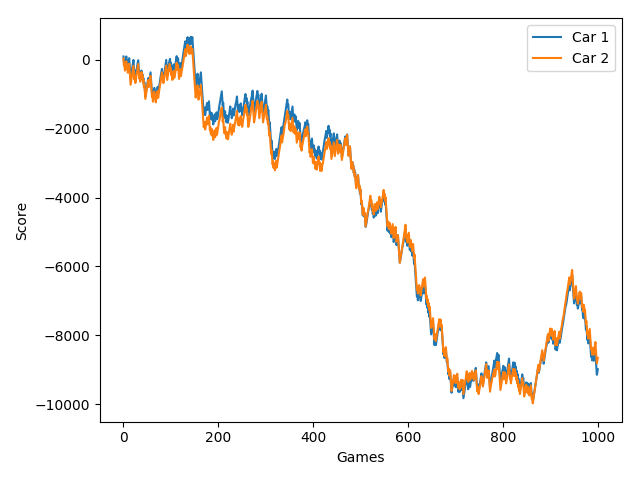
\includegraphics[width=.4\textwidth]{Part1_Random}}
  \caption{Scores for zero intelligence agents and learning agents (respectively) in the first problem.}
  \label{fig:ScoresPart1}
\end{figure}

In \cref{tab:QTablePart1} I have provided one of the possible Q-matrices formed after 1000 turns with each car having a learning factor equal to $0.9$ and discount factor $0.5$.
\begin{table}[htbp]
  \centerline{
    \begin{tabular}{|l|l|l|}
      \hline
      \diagbox{A}{S}& Wait & Drive \\ \hline
      Wait  & -16.67  & 126.67   \\ \hline
      Drive & 53.33  & -203.87   \\ \hline
    \end{tabular}
    \begin{tabular}{|l|l|l|}
      \hline
      \diagbox{A}{S}& Wait & Drive \\ \hline
      Wait  & -13.95  & -203.87   \\ \hline
      Drive & -13.95  & 200.00   \\ \hline
    \end{tabular}}
  \caption{Q matrix for each of the cars in simulation, "submissive" car on the left, "dominant" one on the right.}
  \label{tab:QTablePart1}
\end{table}

Using Q-learning I have also been able to develop a very effective social convention where each car learns not to drive if the bridge is too full and as such it their scores manage to always increase. Increasing $\lambda$ value leads to more cars waiting in line, which causes them to earn lesser score, but they don't affect the overall result. However increasing the number of cars and lowering bridges capacity leads to a surprising result where there is a very visible split among the results. Values used in simulation are: $\lambda: \, 1.5$, number of cars: $15$, $\alpha: \, 0.9$, $\phi: \, 0.66$. Scores for cars in normal situation and with increased number of cars and lowered bridge capacity can be seen in \cref{fig:ScoresPart2}.

\begin{figure}[htbp]
  \centerline{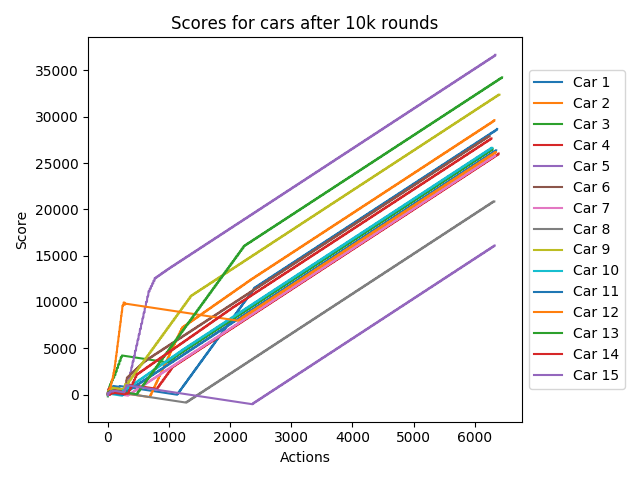
\includegraphics[width=.4\textwidth]{Part2_QLearning}}
  \centerline{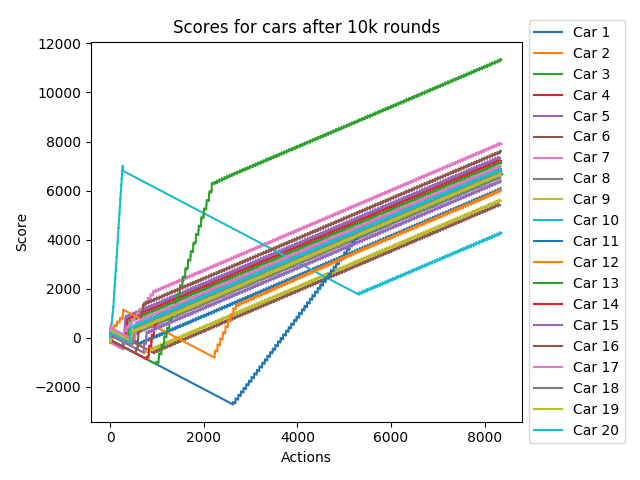
\includegraphics[width=.4\textwidth]{Part2_Curiosity}}
  \caption{Scores for normal case and situation with more cars and lower capacity.}
  \label{fig:ScoresPart2}
\end{figure}

In \cref{tab:QTablePart2} I have provided one of the possible Q-matrices formed after $10000$ rounds by one of the cars. This is of course highly variable and some cars end up with slightly negative values in places other than the last state that would end up to bridge collapse.

\begin{table}[htbp]
  \centerline{
    \begin{tabular}{|l|l|l|l|l|l|l|}
      \hline
      Q-values:          \\ \hline
      3.9617887930067868 \\ \hline
      128.97605980893587 \\ \hline
      68.83724816000003  \\ \hline
      132.72264          \\ \hline
      88.04689076791496  \\ \hline
      -180.0             \\ \hline
    \end{tabular}}
  \caption{Q matrix one of the cars in my simulation.}
  \label{tab:QTablePart2}
\end{table}

In the case of cars driving as taxis I found what's the mean price after each day in the simulation that ran for $1000$ days for both the learning agents and zero intelligence agents. In case of learning agents representing passengers they can be considered as pretty random, since I haven't set up my project to re-use them. In this case once can clearly see that taxi drivers get the upper hand and prices quickly rise up and stay far above prices generated by zero intelligence agents. They also deviate much less than in the case of ZI-agents. Prices are shown in \cref{fig:ScoresPart3}.

Values used in simulation are: $\phi=0.25$

\begin{figure}[htbp]
  \centerline{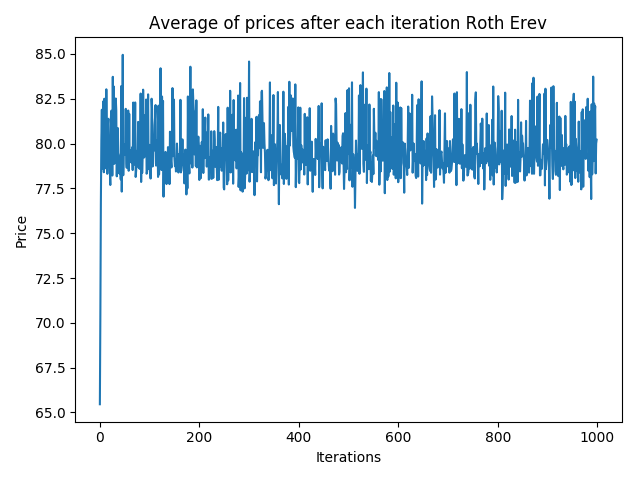
\includegraphics[width=.4\textwidth]{Average_Price_Roth_Erev}}
  \centerline{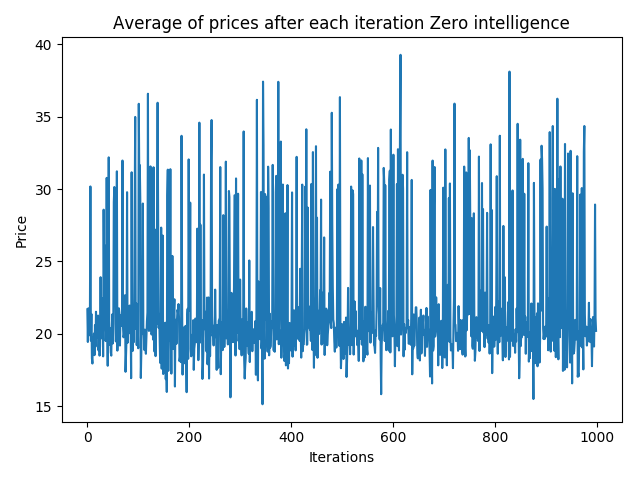
\includegraphics[width=.4\textwidth]{Average_Price_Zero_Int}}
  \caption{Average prices generated by intelligent and random agents over span of $1000$ days.}
  \label{fig:ScoresPart3}
\end{figure}

Resulting propensities always seemed to stop at similar values which are shown in \cref{tab:QTablePart3}

\begin{table}[htbp]
  \centerline{
    \begin{tabular}{|l|l|l|l|l|l|l|}
      \hline
      Lower               & Raise              \\ \hline
      0.41017003892640636 & 0.5898299610735938 \\ \hline
  \end{tabular}}
  \caption{Propensities for taxi after $1000$ days, opposite for passengers.}
  \label{tab:QTablePart3}
\end{table}

\section{Discussion}
As discussed a bit before for the part 1 my cars were able to reach a type of social convention with an "alpha \& beta" mechanic where one car was always dominating the other. I think that if I set up my simulation in another way, where each decision would be independent of the other or employed another learning algorithm I might have reached a more fair situation.

As it is right now with simple maximizing Q-learning, cars will always try to reach best score and in this way learn to cooperate in a way even if one of them is losing to the other. There are some cases where those car take a while to learn to cooperate though, but after $100$ rounds they are guaranteed to start earning points instead of losing them.

In the case of several cars on the bridge, they too learn to stop driving if there are too many cars on the bridge. They learn to keep use the bridge to the fullest, but not collapse it after enough time. In the example shown before where capacity was low and there were many cars we can clearly see a clustering of scores with few outliers. Some cars in this situation are plain lucky and manage to amass a bigger score in the start and keep it, while others are not so lucky and instead lose them and stay poor for the remainder of the simulation. However this is quite random as I choose the cars randomly.

Now if there was another car that wanted to cross the bridge in another way it would have a tough time learning if the bridge was still a one way bridge. As it would most likely collapse it or crash with incoming cars. However if it was a two way bridge with a set capacity I see no problem in it learning to do so if I only had time to implement it. If we're looking at a situation with a two lane bridge I see no problem in cars learning to drive without any problem as it is now. However if this bridge kept being a one way bridge, then the situation would be harder to solve. In this case lack of communication is highly detramental and therefore I would suggest using a learning algorithm that would let agents communicate with each other and cooperate this way.

In the case of last assignment I haven't had time to properly implement it and I doubt that any of us would have a chance to solve both assignments if we hadn't had cooperated on it. In my case I lack a way for my passengers to learn properly therefore what I will talk about here will be highly influenced by those lacking features. 

What I can say for certain is that prices reached by the learning agentsare much more consistent, than those reached by absolutely random agents, even if passengers are pretty much random agents that learn nothing or almost nothing. If both the passengers and taxis would have more time to learn then I am sure that average prices per day would be much more stable, and on daily basis they would increase with demand and lower when there is no much call for taxis. Taxis would most likely benefit from finding out what is the maximum price they can ask for given the demand from passengers and try to aim a bit lower so that they will be chosen more often.

If the number of taxis is not highly disproportional to the number of passengers both the ZI-agents and learning agents are able to clear up the waiting lines. However learning agents do it faster as one can see in the \cref{fig:TakenTaxis}, where $60$ taxis were let loose in the simualtion. It's also worth noting that when demand is high, learning agents are able to better utilize it and almost all taxis were driving when there were a lot of passengers waiting to go home.

\begin{figure}[htbp]
  \centerline{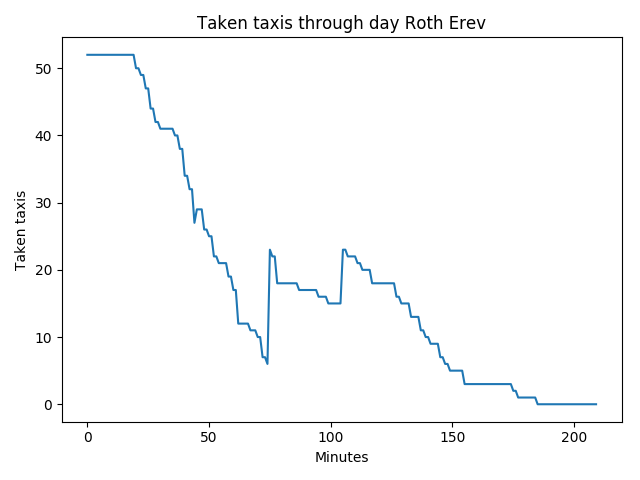
\includegraphics[width=.4\textwidth]{Taken_Taxis_Roth_Erev}}
  \centerline{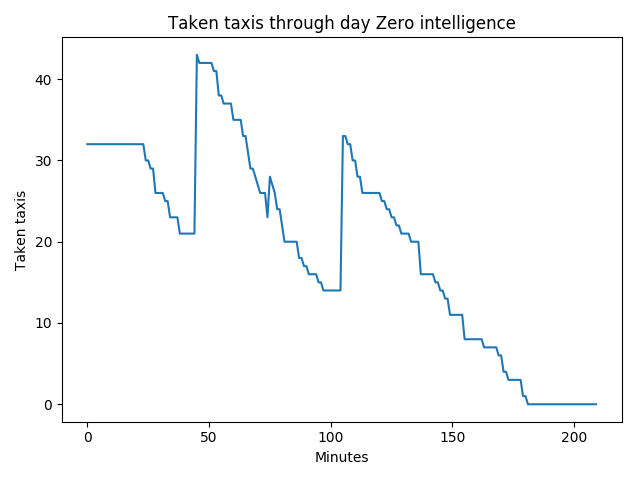
\includegraphics[width=.4\textwidth]{Taken_Taxis_Zero_Int}}
  \caption{Number of taken taxis plotted throughout the day for noth intelligent agents and ZI-agents.}
  \label{fig:TakenTaxis}
\end{figure}

Given enough time I am certain that the system will ballance itself out and will be able to react to changes like more or less taxis/passengers, different closing hours, etc.

\section*{Acknowledgments}
I would like to thank Christopher Kragebøl Hagerup, Kent Arne Larsen, Hans Victor Andersson Lindbäck, and Olav Kjartan Larseng for helping me underway. We brainstormed a lot of ideas on how to solve this problem, and I got a lot of help with task 1.3 from Victor.


\end{document}

